\documentclass[tikz,border=14pt]{standalone}
\usetikzlibrary{positioning,arrows.meta,calc}
\usepackage{amsmath}

\begin{document}
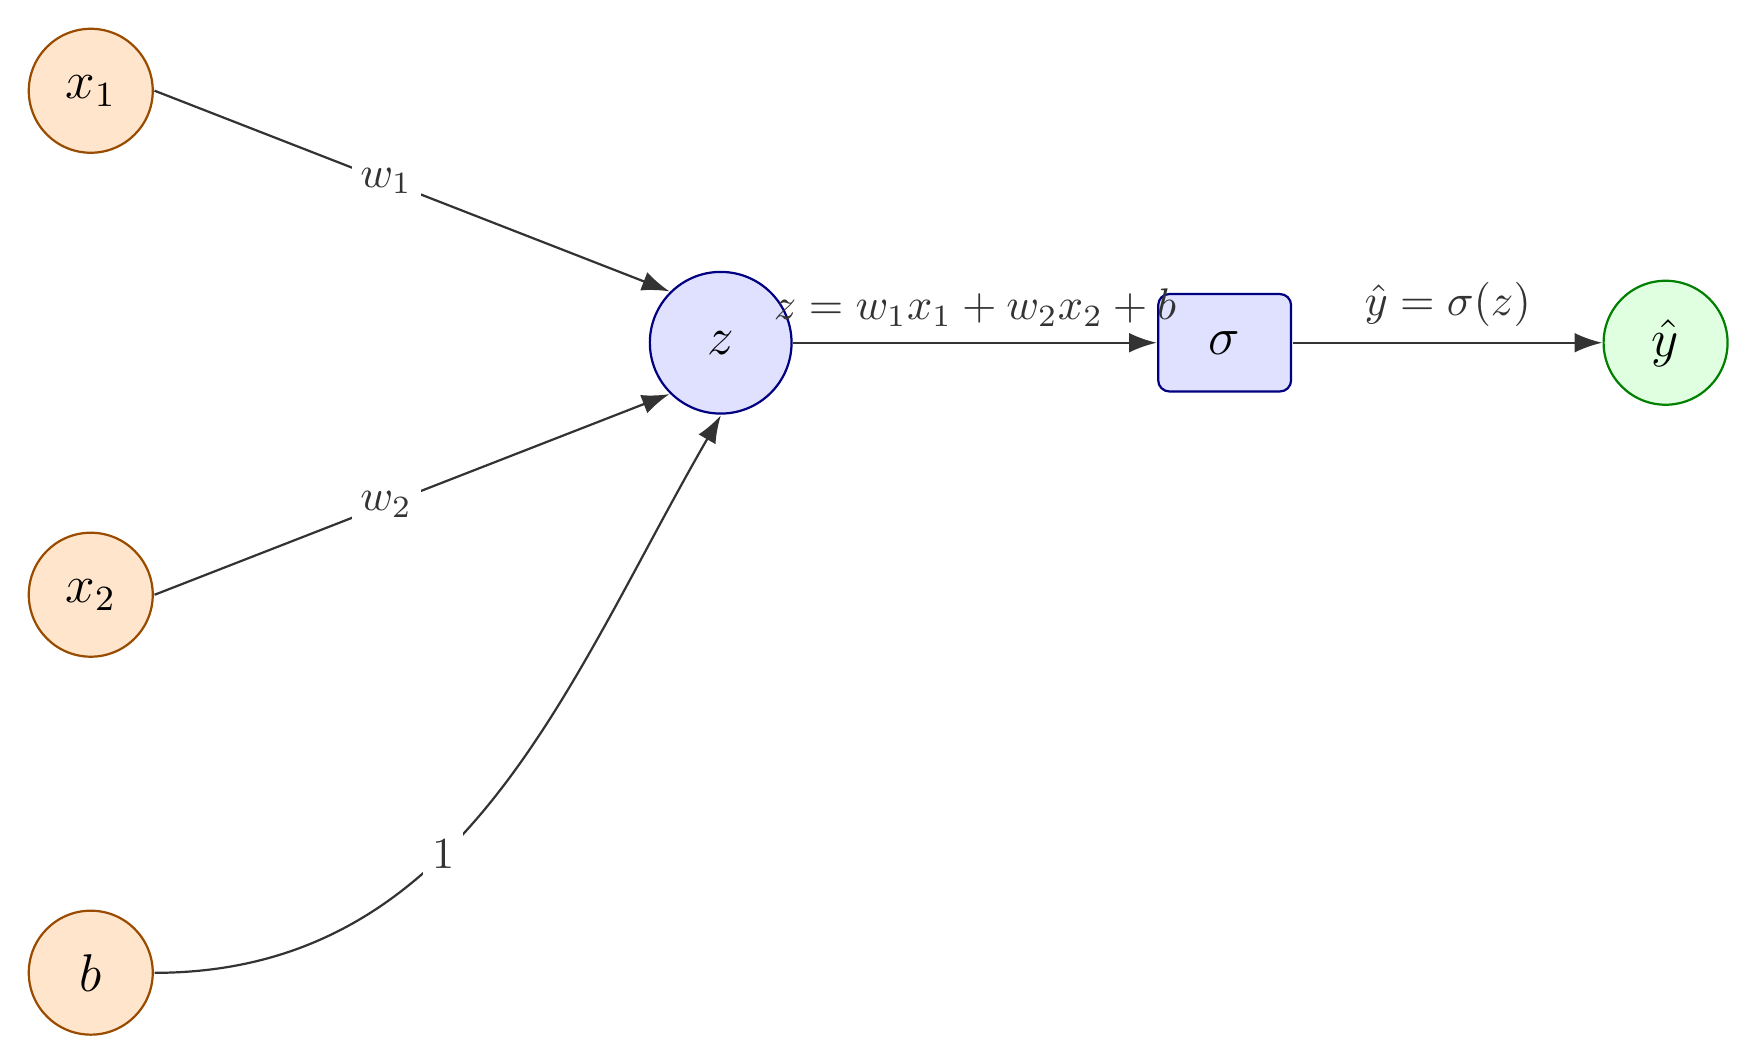
\begin{tikzpicture}[
    scale=1.6, transform shape,
    >=LaTeX,
    input/.style={
        circle,
        minimum width=2.8em,
        draw=orange!60!black,
        fill=orange!20,
        thick,
        font=\large
    },
    bias/.style={
        circle,
        minimum width=2.8em,
        draw=orange!60!black,
        fill=orange!20,
        thick,
        font=\large
    },
    sumnode/.style={
        circle,
        minimum width=3.2em,
        draw=blue!50!black,
        fill=blue!12,
        thick,
        font=\large
    },
    actnode/.style={
        rectangle,
        rounded corners=4pt,
        minimum width=3em,
        minimum height=2.2em,
        draw=blue!50!black,
        fill=blue!12,
        thick,
        font=\large
    },
    output/.style={
        circle,
        minimum width=2.8em,
        draw=green!50!black,
        fill=green!12,
        thick,
        font=\large
    },
    arrow/.style={-{Latex[length=3.5mm, width=2.5mm]}, thick, black!80},
    wlabel/.style={font=\normalsize, fill=white, inner sep=2pt}
]

% --- Nodos de entrada ---
\node[input] (x1) at (0,  2.0) {$x_1$};
\node[input] (x2) at (0, -2.0) {$x_2$};
\node[bias]  (b)  at (0, -5.0) {$b$};

% --- Nodo suma ---
\node[sumnode] (z) at (5.0, 0) {$z$};

% --- Nodo activación ---
\node[actnode] (sigma) at (9.0, 0) {$\sigma$};

% --- Nodo salida ---
\node[output] (yhat) at (12.5, 0) {$\hat{y}$};

% --- Flechas entrada → suma con pesos ---
\draw[arrow] (x1.east) -- (z.north west)
    node[wlabel, pos=0.45] {$w_1$};
\draw[arrow] (x2.east) -- (z.south west)
    node[wlabel, pos=0.45] {$w_2$};
\draw[arrow] (b.east) to[out=0, in=-120]
    node[wlabel, pos=0.4] {$1$}
    (z.south);

% --- Flecha suma → activación ---
\draw[arrow] (z.east) -- (sigma.west)
    node[midway, above, font=\normalsize] {$z = w_1 x_1 + w_2 x_2 + b$};

% --- Flecha activación → salida ---
\draw[arrow] (sigma.east) -- (yhat.west)
    node[midway, above, font=\normalsize] {$\hat{y} = \sigma(z)$};

\end{tikzpicture}
\end{document}
